\section{Evolutionary Algorithm-based Optimization}
\label{sec:optimization}
Once the CHP plant has been modeled by means of the connected NNs, the next step is to  carry out an optimization process to improve the efficiency of the whole process. In particular, we focus on three performance objectives: 1) minimizing the amount of used fuel FG (i.e., natural gas flow), 2) maximizing the generated power POW and 3) maximizing the useful thermal energy FEv (i.e., flow of the fluent in the evaporator). Therefore, we have actually a multi-objective optimization problem. To perform this process, a total of twelve decision variables  are available in the plant; that is, a set of input variables whose values can be changed freely (within certain limits) by the user. These twelve variables are those highlighted in Figure  \ref{fignns}. The mathematical formulation of this multi-objective problem is as follows:
%
\begin{itemize}[-]
	\item Minimize used fuel:		$F_{FlueGas} = F_{Gas_A} + F_{Gas_B} + F_{Gas_C} + F_{Gas_D}$
	\item Maximize drying process: 	$F_{Ev}$
	\item Maximize Power:		$POW = POW_A + POW_B + POW_C + POW_D + POW_{ST}$
\end{itemize}
%
The decision variables and their restrictions are listed below:
%
\begin{itemize}[-]
	\item $T_{B1\_A}, T_{B2\_A}, T_{B1\_B}, T_{B2\_B}, T_{B1\_C}, T_{B2\_C}, T_{B1\_D}, T_{B1\_D}$. (i.e., two air intake temperatures for each engine). $\SI{30}{\celsius} \leq T  \leq  \SI{38}{\celsius}$
	\item $T_{H2O\_Ex}$ (exchange water temperature). $\SI{61}{\celsius}  \leq T  \leq  \SI{65}{\celsius}$
	\item $P_{St\_Gen}$ (pressure of the steam generator). $\SI{20}{bar}  \leq  P  \leq  \SI{22}{bar}$
	\item $P_{Ev}$ (evaporator pressure). $\SI{0.13}{bar}  \leq  P  \leq  \SI{0.17}{bar}$
	\item $T_{H2O\_SH}$ (superheated water temperature). $\SI{110}{\celsius}  \leq  T  \leq  \SI{125}{\celsius}$
\end{itemize}

Our combined approach of using NNs as black box functions may be applied in conjunction with any optimization algorithm that is able to handle real-valued decision variables. For this reason, several state-of-the-art, multiobjective optimization evolutionary algorithms, which all use different search strategies, are considered for solving the proposed optimization problem.

AbYSS (\cite{abyss}) uses a scatter search template as local search operator. ESPEA's (\cite{espea}) niching technique is based on the physical phenomenon of electrostatic potential energy. Indicator-based selection guides the search mechanism of IBEA (\cite{ibea}). MOEA/D (\cite{moead2009}) simultaneously solves multiple scalarized instances of the original problem. NSGA-II (\cite{nsga2}) uses non-dominated sorting and the crowding distance metric. It's successor, NSGA-III (\cite{nsga3part1}), applies a reference point based search method. SMS-EMOA (\cite{smsemoa}) aims at finding a population that maximizes the so-called hypervolume measure. Finally, SMPSO (\cite{smpso}) is a particle swarm optimization approach. We have performed an extensive computational study making use of the jMetal framework version 4.5 (\cite{jmetal2}), in order to assess the performance of these individual algorithms. Our code and resources are hosted online on Sourceforge and are publicly available\footnote{\url{http://sourceforge.net/projects/jmetalbymarlonso/}}.

As stated before, the performance of the CHP plant is influenced by 213 different parameters, of which 60 were found to have a significant impact. While twelve of these parameters may be manipulated by the plant operator as decision variables, there still exist 48 parameters, whose different combinations of values potentially affect the optimization effort. Therefore, we picked a representative sample of 39 parameter combinations from the month February from our data base that serve as different problem instances for a computational study. The aim of this study is identifying the algorithm that performs best across all scenarios. Each algorithm was run 100 times on every test scenario. Algorithm configurations were taken from their original publications. \num{50000} function evaluations were performed per run. Preliminary tests have revealed that the populations of the algorithms assessed in this study become evolutionary stable around \num{50000} evaluations.

The difficulty in solving a multi-objective optimization problem is that there usually exists no single solution that optimizes all goals at the same time. Instead, optimization algorithms aim at finding a representative approximation to the so-called Pareto optimal front. The Pareto front comprises all solutions that can only be improved in one objective by impairing at least one other objective. The idea is that a decision maker chooses a solution to implement from this approximation. The approximation of a Pareto front is graded with respect to two criteria. The points found by an algorithm should be located as close as possible to the Pareto front. At the same time, the approximation should cover the Pareto front in its entirety so the decision maker has full knowledge about the available options. The former aspect is denoted by convergence and the latter by diversity (\cite{basicDeb,basicCoello}).

We chose the Inverted Generational Distance (IGD) as performance metric, since it captures both convergence and diversity (\cite{van1998evolutionary}). The IGD metric computes the average of the minimum distances of every Pareto optimal point to a given Pareto front approximation. Since the Pareto fronts are not known in our case, we use all nondominated solutions obtained across all algorithm runs of a single problem instance as reference front. Objective values were normalized to mitigate the effect of different scalings.

A preliminary analysis has revealed that the performance of an individual algorithm only differs marginally across the different problem instances. This observation indicates that our approach is very robust with respect to the parameters that cannot be influenced by the operator. For the sake of clarity, we therefore only provide a summary of the results in Table \ref{tbl:summary}. Full results are provided in the appendix in Table \ref{table:median.IGD}.

\begin{table}
\caption{Mean and standard deviation of median IGD across all test problems.}
\label{tbl:summary}
\centering
\begin{tabular}{*{4}{c}} \toprule
AbYSS & ESPEA & IBEA & MOEAD\\ \cmidrule(lr){1-1} \cmidrule(lr){2-2} \cmidrule(lr){3-3} \cmidrule(lr){4-4}
$\num{3.41E-4}_{\num{2.13E-5}}$ & $\num{1.69e-4}_{\num{1.92e-5}}$ & $\num{1.53E-3}_{\num{1.88E-4}}$ & $\num{1.51E-3}_{\num{1.72E-4}}$ \\ \midrule
NSGA-II & NSGA-III & SMPSO & SMS-EMOA \\ \cmidrule(lr){1-1} \cmidrule(lr){2-2} \cmidrule(lr){3-3} \cmidrule(lr){4-4}
$\num{3.55E-4}_{\num{2.20E-5}}$ & $\num{1.25E-3}_{\num{1.33E-4}}$ & $\num{3.30E-4}_{\num{2.07E-5}}$ & $\num{1.53E-3}_{\num{1.68E-4}}$ \\
\bottomrule
\end{tabular}
\end{table}

The study results demonstrate that there exist clear performance differences between individual algorithms. Values of the IGD metric differ by a factor of ten from best to worst. This implies that the choice of algorithm greatly influences the optimization outcome. Best results are obtained using ESPEA, whereas AbYSS, NSGA-II and SMPSO show also good performances. IBEA, MOEA/D, NSGA-III and SMS-EMOA, on the other hand, trail behind. The smallest average IGD is achieved by ESPEA. A Kruskal-Wallis test (\cite{kruskal1952use}) in conjunction with a post-hoc analysis has revealed that the difference in IGD values between ESPEA and the other algorithms across al 39 problems is significant.\footnote{P-values were equal to zero in our analysis.}

\begin{figure}
\centering
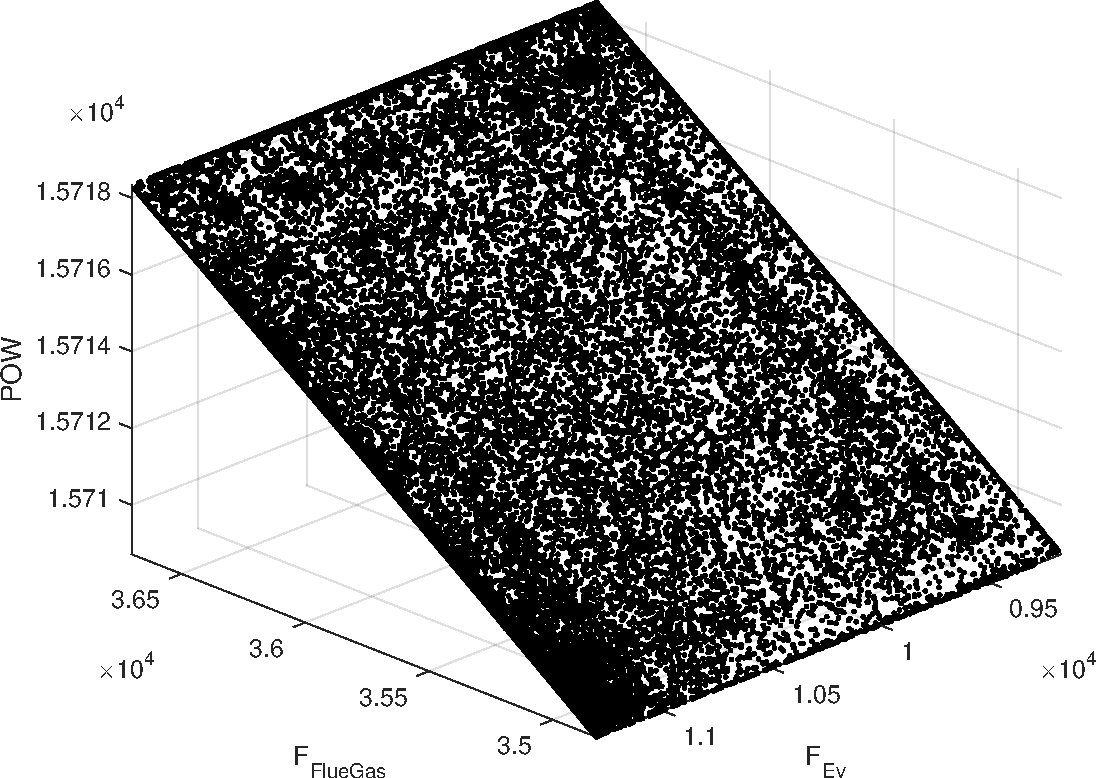
\includegraphics[width=0.7\textwidth]{figures/paretofront_cropped.pdf}
\caption{Pareto front of problem instance two out of 39 of the cogeneration optimization problem. The front is a collection of all non-dominated solutions computed during the study.}
\label{fig:paretofront}
\end{figure}

A closer analysis of the Pareto front reveals possible explanations for the performance differences observed. Figure \ref{fig:paretofront} shows the Pareto front of a cogeneration optimization problem instance. The rectangular shape of the front suggests that all Pareto optimal points lie on a plane. A regression analysis has indeed confirmed that for 38 out of 39 problem instances all points can be fitted in a plane with a coefficient of determination of one.\footnote{The Pareto front of instance one out 39 (referenced as CG0 in Table \ref{table:median.IGD}) consists of two different planes.} Strikingly, the Pareto front is linear, whereas the problem itself is not.

\begin{figure}
\centering
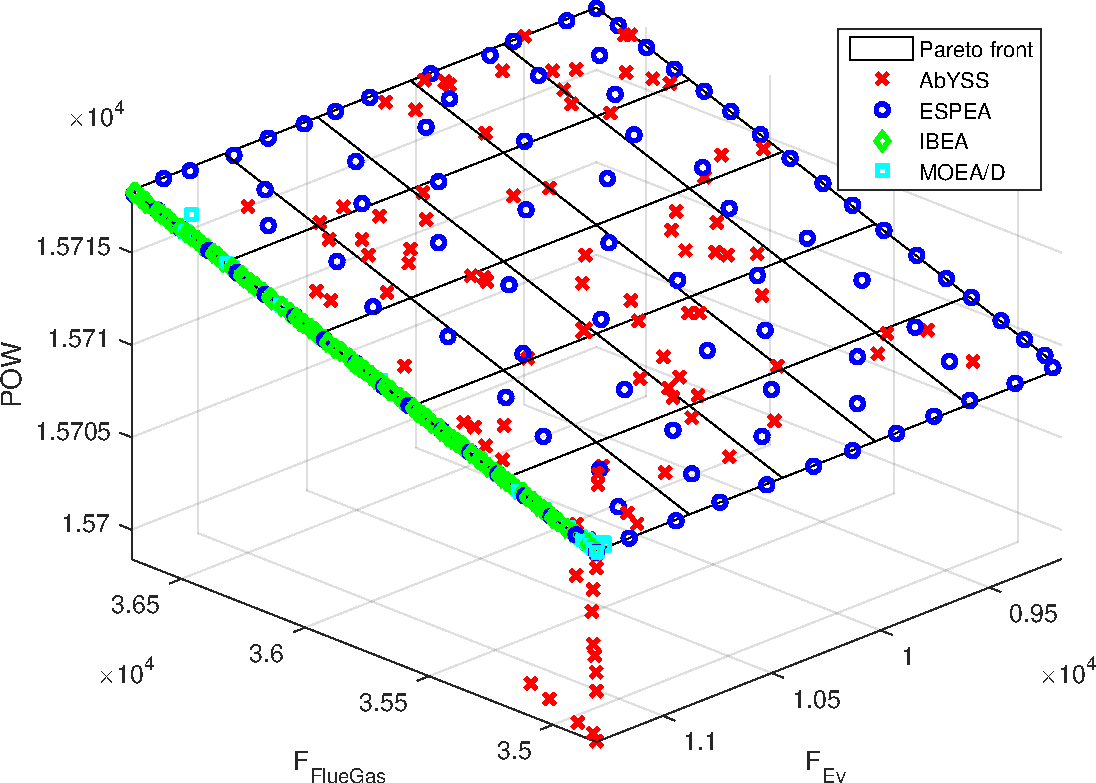
\includegraphics[width=0.7\textwidth]{figures/example1_cropped.pdf}
\caption{Representative search results of the algorithms AbYSS, ESPEA, IBEA and MOEA/D for illustrating their performance.}
\label{fig:exruns1}
\end{figure}

Figures \ref{fig:exruns1} and \ref{fig:exruns2} offer an explanation to why algorithm performances can be divided into two tiers. AbYSS, ESPEA, NSGA-II and SMPSO capture the Pareto front in its entirety, whereas ESPEA achieves the most equidistant approximation. NSGA-II and AbYSS additionally retrieve dominated points as indicated in the plot. IBEA, MOEA/D, NSGA-III and SMS-EMOA focus mainly on a single edge of the front. We believe that using reference points from \cite{nbi} as it is suggested by \cite{moead2009,nsga3part1} is problematic given the presented front. We assume that the reference points do not cover the front equally, which leads to a strong focus on boundary solution. A better choice of reference points might ameliorate this issue. Hypervolume-based methods such as SMS-EMOA and the IBEA configuration used in this study, seem to struggle with the geometry of the front. We speculate that, despite objective normalization, boundary points yield the highest hypervolume contributions on plane-shaped fronts. Although the figures only depict single runs, these basic observations could be confirmed for other problem instances and different runs as well.

\begin{figure}
\centering
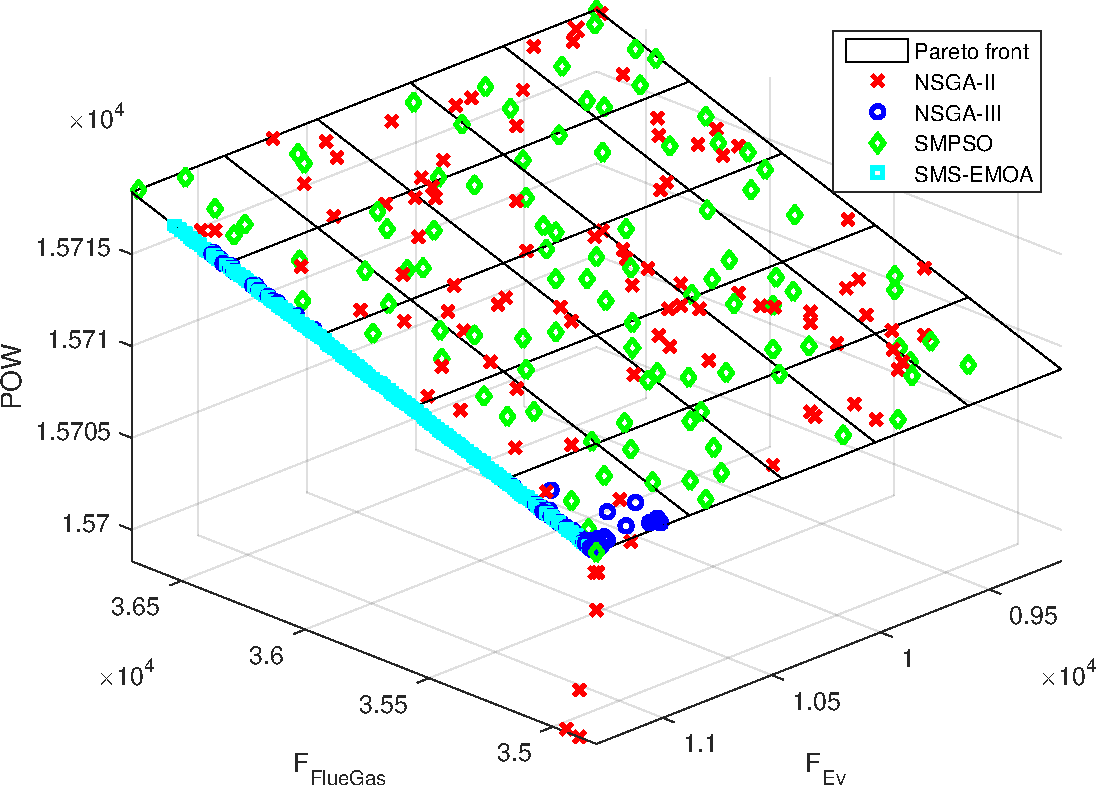
\includegraphics[width=0.7\textwidth]{figures/example2_cropped.pdf}
\caption{Representative search results of the algorithms NSGA-II, NSGA-III, SMPSO and SMS-EMOA for illustrating their performance.}
\label{fig:exruns2}
\end{figure}

Robustness is another aspect of algorithm performance that is of interest in our setting. In practice, it is usually not feasible to conduct 100 runs and choose the most preferable option from this pool of alternatives. If there is little variability between the results of individual runs, however, we can conclude that every single run yields a satisfying result. One way of assessing robustness is considering the surface attainment (\cite{fonseca1996performance}) across multiple runs. Surface attainment measures the space that is dominated by a given approximation set. When measured across multiple runs, surface attainment yields the space that is dominated in a given percentage of runs. Figure \ref{fig:surfaceattainment} compares the first and 100th percentile of problem instance \textit{CG1}. We can see that both surfaces nearly coincide, further indicating that our optimization approach is very robust across different runs. Identical observations were made for other problem instances as well.

\begin{figure}
	\begin{subfigure}{0.47\textwidth}
	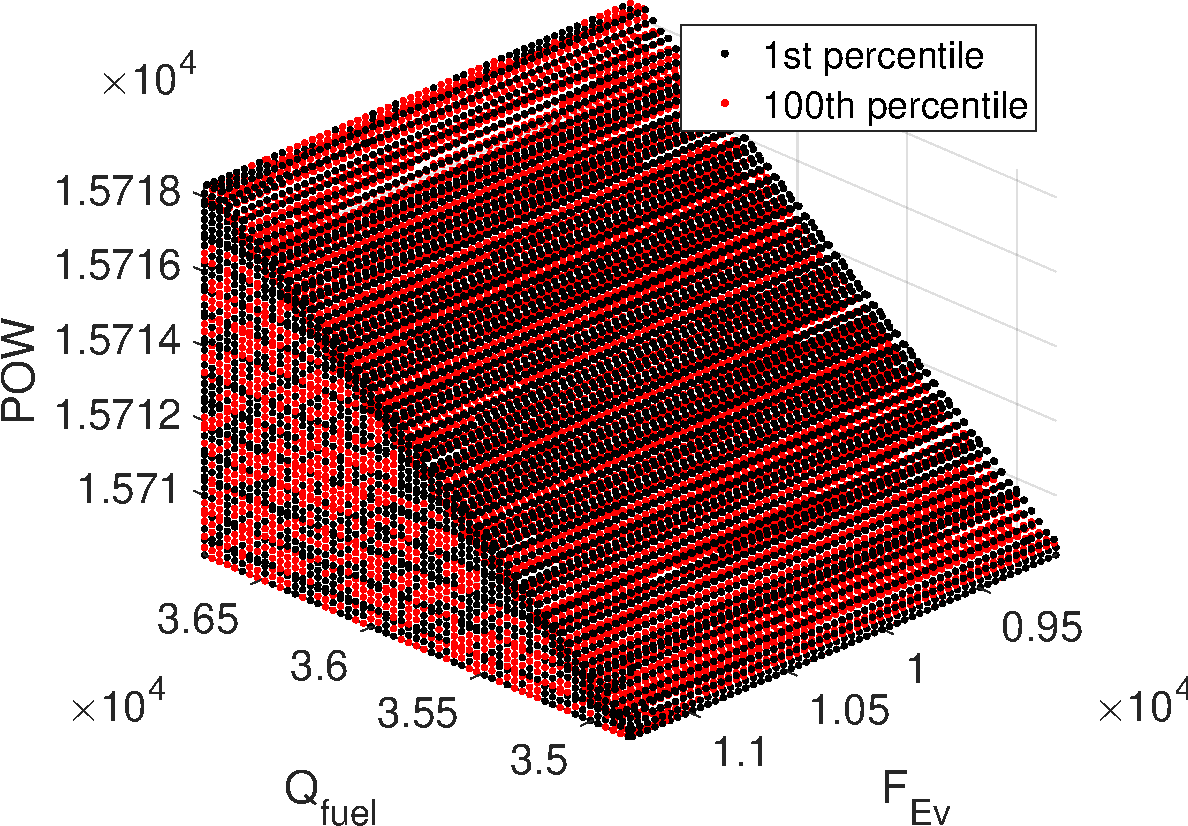
\includegraphics[width=\textwidth]{figures/safront_cropped.pdf}
	\end{subfigure}
\hfill
	\begin{subfigure}{0.47\textwidth}
	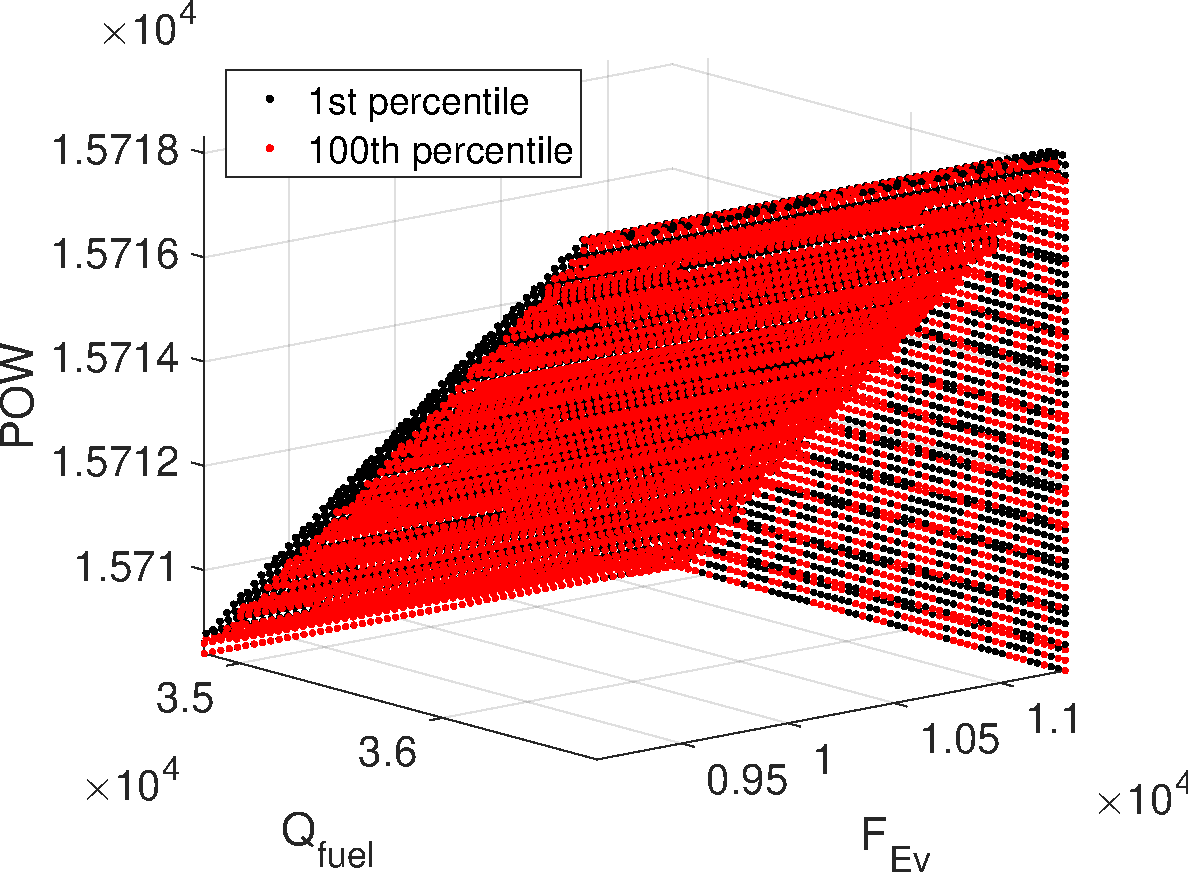
\includegraphics[width=\textwidth]{figures/saback_cropped.pdf}
	\end{subfigure}
\caption{Surface attainment plot of ESPEA for the first and 100th percentile for problem instance \textit{CG1}. The first percentile depicts the space that is dominated by all ESPEA runs combined, while the 100th percentile shows the space that is dominated in all of the 100 runs.}
\label{fig:surfaceattainment}
\end{figure}

The multi-objective approach generates a set of solutions among which a decision maker chooses an option that fits his preferences best. In the present context, there exists an efficiency measure that may be used to evaluate the quality of the cogeneration process. Efficiency can be defined as a quotient of the power generated by the unused energy contained in the flue gases:
%
\begin{equation}
\label{eq:efficiency}
\varepsilon_{EE} = \frac{100 \cdot POW}{F_{FlueGas} - F_{Ev}/0.9}.
\end{equation}
%
A question that needs to be addressed in this context is, whether the multi-objective approach is suited to find a solution that maximizes the efficiency of the cogeneration process. Our computational study has revealed that all algorithms with the exception of NSGA-II and NSGA-III were able to find a solution possessing an efficiency of 70.6 on every problem instance in their median runs. The best solutions obtained by NSGA-II and NSGA-III across all problems exhibit an efficiency of 70.5. Both values are higher than any efficiencies achieved by previous optimization efforts, where values varied largely between 61 and 70 (\cite[Fig. 11]{Seijo2016309}).

If a choice rule such as (\ref{eq:efficiency}) is given, it makes sense to focus the search from the beginning on those regions of the Pareto front that yield the highest efficiency. In a multi-objective context, however, a decision maker is usually not only interest in obtaining a preconceived optimum, but also in comparing his choice to other options available (\cite{roy1996multicriteria,kahneman1979prospect}).

ESPEA provides a mechanism that bridges the gap between those conflicting goals. The basic notion of this algorithm consists of interpreting the Pareto front as closed physical system in which charged particles, represented by solutions, may move freely. The aim of ESPEA is to obtain an approximation of a fixed, given size of the Pareto front that minimizes the energy of the system. For this purpose, the algorithm maintains an archive of non-dominated solutions. The energy of the archive is computed as the sum of all pair-wise energies between individual solutions of the archive. In physics, the electrostatic energy that works between two particles is the product of their charges divided by their Euclidean distance. ESPEA uses the distance in objective space for computing energies. Charges are interpreted as utility values, where a lower utility corresponds to a higher desirability. In case all solutions are equally desirable, charges are set to one, as it was done for the computational study. In the second part of our analysis, we use (\ref{eq:efficiency}) as charges for biasing the search towards the efficiency optimum. Efficiency values were raised by three to increase the bias of the search as hinted at \cite{espea}.

\begin{figure}
\centering
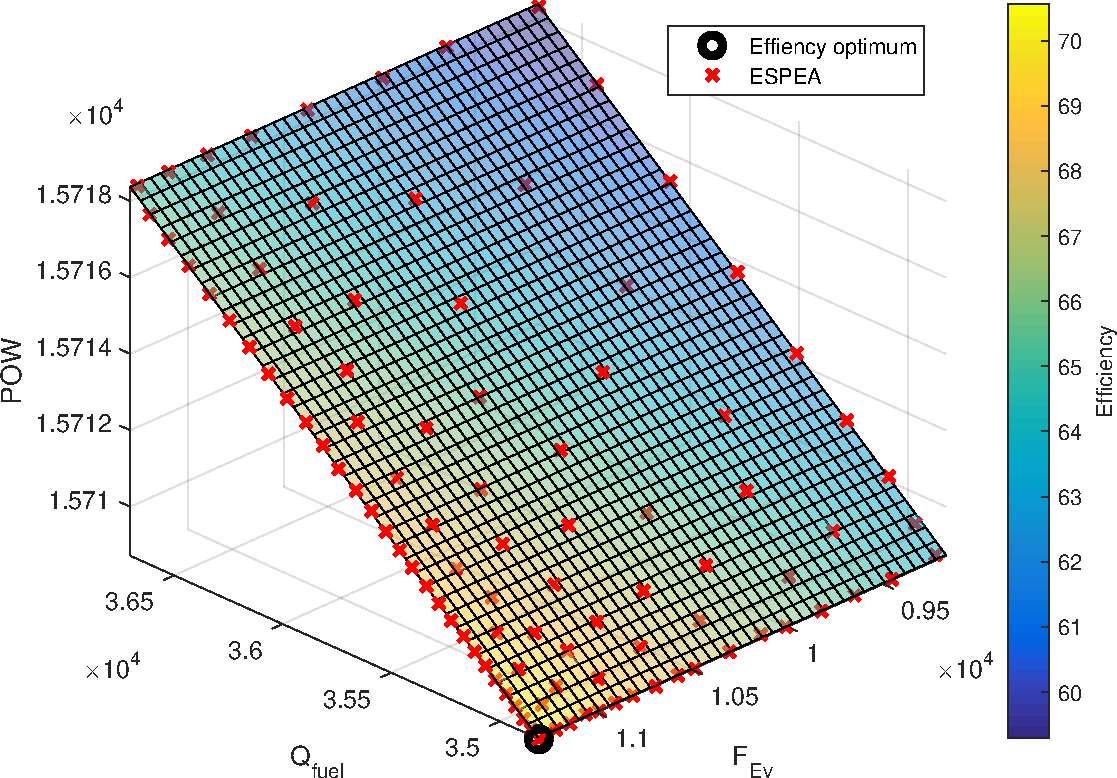
\includegraphics[width=0.7\textwidth]{figures/espeacharge_cropped.pdf}
\caption{ESPEA run using effiency values as charges.}
\label{fig:espea}
\end{figure}

Figure \ref{fig:espea} illustrates the effect of using the charge mechanism in ESPEA. We observe that the density of solutions is higher in those regions that show high efficiencies. At the same time, a focus on the entire front is retained enabling the decision maker to compare is favorite choice with other alternatives.

Since the cogeneration optimization problem as presented in this work is embedded in a real-time application, algorithm run times are a critical issue in this context. The CHP is expected to be reconfigured every 15 minutes according to the currently observed parameter values. A single algorithm run should therefore take considerably less than 15 minutes on commercial off-the-shelf medium-class computer hardware. With the exception of ESPEA and SMS-EMOA, all algorithms finish \num{50000} within less than ten seconds on an Intel Core i5-4300U processor running Windows 8.1. A single ESPEA runs takes about half a minute, whereas an SMS-EMOA execution can take up to ten minutes. Although run-times also highly depend on the implementation and the chosen programming language, the most important factor is the computational complexity of executing a single iteration of a given optimization algorithm. ESPEA and SMS-EMOA are steady-state algorithms implying that more costly operations are performed per function evaluation. Additionally, SMS-EMOA solves an NP-hard problem during each iteration (\cite{hypervolumecontribution}), which results in a very high run-time. Considering all this, we may draw the conclusion that every algorithm assessed in this study is suitable for an on-line implementation with the exception of SMS-EMOA.

%____________________________________
